\documentclass[11pt]{article}
\usepackage[a4paper, total={6in, 10in}]{geometry}
\usepackage{graphicx}
\usepackage{amsmath,amsfonts,amssymb}
\usepackage{listings}
\usepackage{booktabs}
\usepackage[T1]{fontenc}
\usepackage{color}
\usepackage{minted}
\usepackage[colorlinks=true, linkcolor=blue, urlcolor=blue, citecolor=blue,
  pdfborder={0 0 255}]{hyperref}
\usepackage{colortbl}
\usepackage{url}
\usepackage{xcolor}
\usepackage{caption}
\usepackage{subcaption}
\usepackage{dirtytalk}
\usepackage[semicolon, round]{natbib}
\usepackage[ruled]{algorithm2e}
\usepackage{multirow}
\usepackage{setspace}
\usepackage{placeins}
\captionsetup[table]{skip=10pt}
\renewcommand{\vec}[1]{\mathbf{#1}}
\SetKwComment{Comment}{$\triangleright$\ }{}
\hypersetup{%
	colorlinks=true,
	linkcolor=blue,
	linkbordercolor={0 0 1}
}

% \renewcommand\lstlistingname{Algorithm}
% \renewcommand\lstlistlistingname{Algorithms}
% \def\lstlistingautorefname{Alg.}

% \lstdefinestyle{Python}{
% 	language        = Python,
% 	frame           = lines,
% 	basicstyle      = \footnotesize,
% 	keywordstyle    = \color{blue},
% 	stringstyle     = \color{green},
% 	commentstyle    = \color{red}\ttfamily
% }

\setlength{\parindent}{0.0in}
\setlength{\parskip}{0.02in}

\newcommand{\argmin}{\mathop{\mathrm{argmin}}}
\newcommand{\argmax}{\mathop{\mathrm{argmax}}}
\newcommand{\minimize}{\mathop{\mathrm{minimize}}}
\newcommand{\maximize}{\mathop{\mathrm{maximize}}}
\newcommand{\st}{\mathop{\mathrm{subject\,\,to}}}
\newcommand{\dist}{\mathop{\mathrm{dist}}}
\newcommand{\norm}[1]{\left\lVert#1\right\rVert}

\renewcommand{\tt}[1]{\texttt{#1}}
% \renewcommand{\vec}[1]{\mathbf{#1}}

\DeclareCaptionType{codelisting}[Listing][List of mytype]
\newenvironment{codeblock}{\captionsetup{type=codelisting}}{}

\def\R{\mathbb{R}}
\def\E{\mathbb{E}}
\def\P{\mathbb{P}}
\def\S{\mathbb{S}}
\def\Cov{\mathrm{Cov}}
\def\Var{\mathrm{Var}}
\def\half{\frac{1}{2}}
\def\quat{\frac{1}{4}}
\def\sign{\mathrm{sign}}
\def\supp{\mathrm{supp}}
\def\th{\mathrm{th}}
\def\tr{\mathrm{tr}}
\def\dim{\mathrm{dim}}
\def\dom{\mathrm{dom}}
\def\th{$^{\mathrm{th}}$}

\title{EE2003 Assignment 2 \vspace{-1em}}
\author{Niranjan A. Kartha, EE21B095\vspace{-3em}}
\date{}

\begin{document}
\maketitle
\section*{P32. Restoring Division}
Design a Verilog module that implements the restoring division algorithm. The module should take two 8-bit unsigned numbers (\tt{dividend} and \tt{divisor}) as inputs and produce an 8-bit quotient \tt{quotient} and an 8-bit remainder \tt{remainder}.

\subsection*{Implementation}
Two extra inputs, \tt{clk} and \tt{reset} have been introduced in order to control the module. The \tt{reset} bit should be set high for one clock cycle once the inputs to the module are loaded. An output bit, \tt{ready}, is set high when the computation is complete.

Two extra registers, \tt{state} and \tt{rold}, are used. The \tt{state} register keeps track of how many bits have been divided, and \tt{rold} is used to left-rotate the \tt{dividend} to append bits to the partial \tt{remainder}.

After the inputs have been loaded, \tt{quotient} and \tt{remainder} become ready after 7 clock cycles.

\subsection*{Source code}

\begin{codeblock}
\inputminted[breaklines,
 mathescape,
 linenos,
 numbersep=5pt,
 frame=single,
 xleftmargin=0pt]{verilog}{divider/divider.srcs/sources_1/new/divider.v}
\end{codeblock}

\subsection*{Testbench}

\begin{codeblock}
\inputminted[breaklines,
 mathescape,
 linenos,
 numbersep=5pt,
 frame=single,
 xleftmargin=0pt]{verilog}{divider/divider.srcs/sim_1/new/divider_tb.v}
\end{codeblock}

\subsection*{Outputs}
Input 1 shows $144 / 12 = 4$ with remainder $0$. Input 2 shows $255/4 = 63$ with remainder $3$.
\begin{figure}[H]
\centering
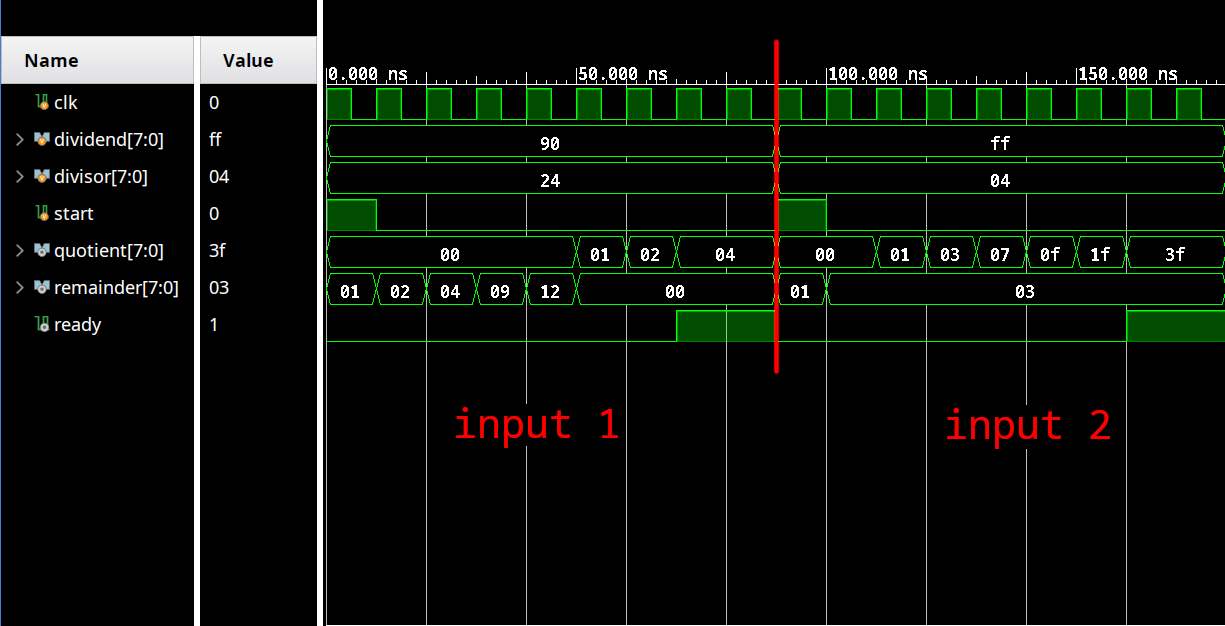
\includegraphics[width=\linewidth]{output.png}
\end{figure}

\end{document}
